\documentclass[12pt,a4paper]{article}

\usepackage{amsfonts}
\usepackage{amssymb}
\usepackage{amsmath}
\usepackage{amsthm}
\usepackage{enumerate}

\usepackage[utf8]{inputenc}
\usepackage{csquotes}
\usepackage{polski}
\usepackage[utf8]{inputenc} 
\usepackage[T1]{fontenc}
\usepackage{indentfirst}

\usepackage{hyperref}

\usepackage{tikz}
\usetikzlibrary{arrows}

\frenchspacing

%\renewcommand{\arraystretch}{3.0}
%\renewcommand{\thefootnote}{\fnsymbol{footnote}}

% Makro do automatycznego tworzenia wektorów/macierzy dowolnego wymiaru,
% potem można pomyśleć o stworzeniu biblioteczki z przydatnymi rzeczami.
\newcount\colveccount
\newcommand*\colvec[1]{
        \global\colveccount#1
        \begin{pmatrix}
        \colvecnext
}
\def\colvecnext#1{
        #1
        \global\advance\colveccount-1
        \ifnum\colveccount>0
                \\
                \expandafter\colvecnext
        \else
                \end{pmatrix}
        \fi
}

\newcommand{\norm}[1]{\left\lVert#1\right\rVert}

% Pisanie za każdym razem \mathbb{R} jest zbyt długie, teraz wystarczy \RR.
\newcommand{\RR}{\mathbb{R}}
% tak samo \overrightarrow
\newcommand{\V}[1]{\overrightarrow{#1}}
\newcommand{\Pair}[2]{\left<#1,#2\right>}
\renewcommand{\qed}{$\square$}

% Definicja stylów:
\theoremstyle{plain}
\newtheorem{tw}{Twierdzenie}[section]
\theoremstyle{definition}
\newtheorem{ft}{Fakt}[section]
\theoremstyle{definition}
\newtheorem{df}{Definicja}[section]
\theoremstyle{definition}
\newtheorem*{nt}{Notacja}
\theoremstyle{definition}
\newtheorem*{dd}{Dowód}
\theoremstyle{definition}
\newtheorem*{prz}{Przykład}

\begin{document}

\section{Przestrzeń $\RR^2$ i $\RR^3$} % wykład 1, 21.02.2019

\begin{df}[geometryczna]
  Wektor definiujemy jako uporządkowaną parę punktów $\Pair{A}{B}$ w przestrzeni $\RR^2$/$\RR^3$ i oznaczamy $\V{AB}.$
\end{df}

Dla wektora $\V{AB}$ definiujemy następujące pojęcia:
\begin{itemize}
  \item długość --- odległość z punktu $A$ do $B;$
  \item kierunek --- kierunek wyznaczany przez prostą przechodzącą przez punkty $A$ i $B;$
  \item zwrot --- określamy tylko dla wektorów o tym samym kierunku, dwa wektory mają ten sam zwrot wtedy i tylko wtedy, gdy są skierowane w tą samą stronę. % XD
\end{itemize}

Wektory $\V{AB}$ i $\V{CD}$ uznajemy za równe jeśli mają tą samą długość, kierunek i zwrot.

Wektory mogą być swobodne lub zaczepione\footnote{Wektory zaczepione w sumie nas nie interesują, ale warto pamiętać, że mają one swoje zastowanie, np. w fizyce.}.

W algebrze liniowej zazwyczaj utożsamiamy wektor $\V{OA}$ z punktem $A$, a za początek układu współrzędnych przyjmujemy wektor $O=\colvec{1}{0 \\ 0}.$

\begin{ft} Dla dowolnego wektora $\V{AB}$ zachodzi: $\V{AB} = B - A.$ \end{ft}

\begin{center}
  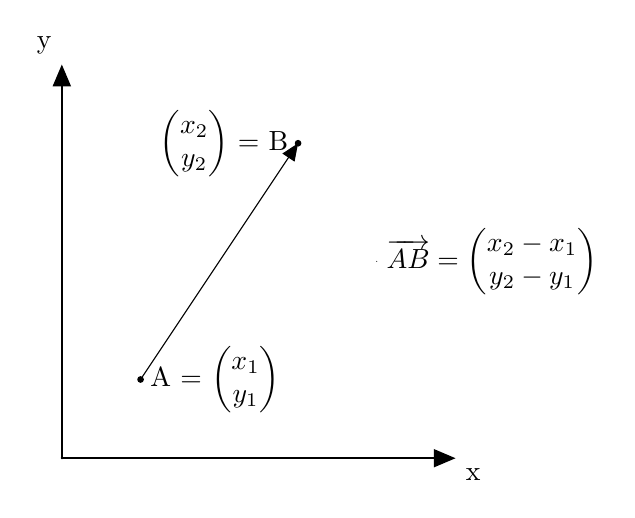
\begin{tikzpicture}[line cap=round,line join=round,>=triangle 45,scale=1,font=\normalsize]
    \draw[thick,->] (0,0) -- (5,0) node[anchor=north west] {x};
    \draw[thick,->] (0,0) -- (0,5) node[anchor=south east] {y};
    \filldraw[black] (1,1) circle (1pt) node[anchor=west] {A = $\colvec{1}{x_1 \\ y_1}$};
    \filldraw[black] (3,4) circle (1pt) node[anchor=east] {$\colvec{1}{x_2 \\ y_2}$ = B};
    \draw[->] (1,1) -- (3,4);
    \filldraw[black] (4,2.5) circle (0pt) node[anchor=west] {$ \V{AB} = \colvec{1}{x_2 - x_1 \\ y_2 - y_1}$};
  \end{tikzpicture}
\end{center}

\begin{df}[algebraiczna]
  Wektor w $\RR^2$ (lub odpowiednio w $\RR^3$) to uporządkowana para (trójka) liczb rzeczywistych.
\end{df}

\begin{nt}
  Dla wygody wektory będziemy zapisywać w kolumnie: $\colvec{1}{x \\ y} \text{lub} \colvec{1}{x \\ y \\ z}.$
\end{nt}

\begin{minipage}[c]{0.70\textwidth}
  \vspace{3mm}
  Na wektorach w $\RR^2$ definiujemy dwa podstawowe działania:
  \begin{itemize}
    \item \emph{(dodawanie wektorów)} $$\colvec{1}{x \\ y} + \colvec{1}{x' \\ y'} = \colvec{1}{x + x' \\ y + y'},$$
    \item \emph{(mnożenie przez skalar)} $$t\colvec{1}{x \\ y} = \colvec{1}{ tx \\ ty }.$$
  \end{itemize}
\end{minipage}
\begin{minipage}[c]{0.30\textwidth}
  \vspace{3mm}
  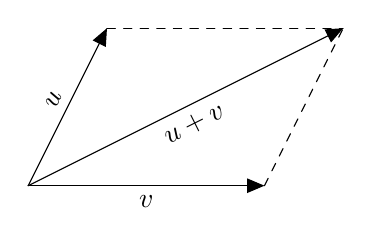
\begin{tikzpicture}[line cap=round,line join=round,>=triangle 45,scale=1,font=\normalsize]
    \draw[->] (0,0) -- (1,2) node[midway,sloped,above] {$u$};
    \draw[->] (0,0) -- (3,0) node[midway,sloped,below] {$v$};
    \draw[dashed] (1,2) -- (4,2);
    \draw[dashed] (3,0) -- (4,2);
    \draw[->] (0,0) -- (4,2) node[midway,sloped,below] {$u+v$};
  \end{tikzpicture} \\
  \small{Zasada równoległoboku} \\\\
  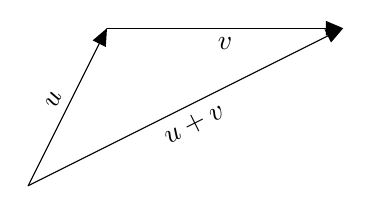
\begin{tikzpicture}[line cap=round,line join=round,>=triangle 45,scale=1,font=\normalsize]
    \draw[->] (5,0) -- (6,2) node[midway,sloped,above] {$u$};
    \draw[->] (6,2) -- (9,2) node[midway,sloped,below] {$v$};
    \draw[->] (5,0) -- (9,2) node[midway,sloped,below] {$u+v$};
  \end{tikzpicture} \\ \small{Zasada trójkąta}
\end{minipage}
\vspace{4mm}

Własności dodawania oraz mnożenia wektorów w $\RR^2 \text{ i } \RR^3$:
\begin{enumerate}[{(}1{)}]
    \item $\forall u, v, w \in \mathbb{R}^2 \quad (u+v)+w = u+(v+w) $
    \item $\forall u, v \in \mathbb{R}^2 \quad u+v = v+u$
    \item $\exists O \in \mathbb{R}^2 \  \forall v \in \mathbb{R}^2 \quad O+v = v+O = v$
    \item $\forall v \in \mathbb{R}^2 \ \exists \text{-} v \in \mathbb{R}^2 \quad v+( \text{-}v) = \text{-} v+v = O$
    \item $\forall u \in \mathbb{R}^2 \ \forall t,s \in \mathbb{R} \quad t(su) = (ts)u$
    \item $\forall u,v \in \mathbb{R}^2 \ \forall t \in \mathbb{R} \quad t(u+v) = tu + tv$ \\ 
          $\forall u \in \mathbb{R}^2 \ \forall t,s  \in
          \mathbb{R} \quad (t+s)u = tu + su$
    \item $\forall u \in \mathbb{R}^2 \quad 1u = u$
\end{enumerate}

\begin{nt} Wektory bazowe będziemy oznaczać jako: $e_1 = \colvec{1}{1 \\ 0}$ i $e_2 = \colvec{1}{0 \\ 1}.$ \end{nt}
\begin{ft} Każdy wektor w $\RR^2$ zapisuje się jednoznacznie jako kombinacja liniowa wektorów bazowych: $a e_1 + b e_2$ dla pewnych liczb $a$ i $b.$ \end{ft}

\begin{df}[algebraiczna]
  Iloczynem skalarnym nazywamy funkcję określoną na $\circ\colon\RR^2\times\RR^2\mapsto\RR$ i zadaną wzorem $\colvec{1}{x \\ y}\circ\colvec{1}{x' \\ y'} = xx' + yy'.$
\end{df}

Własności iloczynu skalarnego:
\begin{enumerate}[{(}1{)}]
  \item $ \forall u, v \in \RR^2 \ u \circ v = 0 \iff u \perp v$ \emph{(przyjmujemy, że wektor $0$ jest prostopadły do każdego wektora),}
  \item $ \forall u, v \in \RR^2 \ u \circ v = v \circ u,$
  \item $ \forall u, v \in \RR^2 \ \forall t \in \RR \ (tu) \circ v =  t(v \circ u),$
  \item $ \forall u, v, w \in \RR^2 \ u \circ (v + w) = u \circ v + u \circ w$
\end{enumerate}

Własności 2, 3, 4 są oczywiste i wynikają wprost z definicji iloczynu skalarnego, natomiast własność 1 najłatwiej jest pokazać korzystając z definicji geometrycznej iloczynu skalarnego.

\begin{df}[geometryczna] Iloczyn skalarny można zapisać także w postaci: $$u \circ v = \norm{u}\norm{v}\cos\sphericalangle(u, v).$$ \end{df}

\begin{tw} Definicja algebraiczna iloczynu skalarnego jest równoważna definicji geometrycznej. \end{tw}

\begin{dd}
  Weźmy dowolne dwa wektory $u = ae_1 + be_2$ i $v = a'e_1 + b'e_2$. Łatwo sprawdzić, że obie definicje spełniają własności 2, 3 i 4, zatem przekształćmy ich iloczyn skalarny: \begin{align*}u \circ v &= (ae_1 + be_2) \circ (a'e_1 + b'e_2) \\ &= aa'(e_1 \circ e_1) + ab'(e_1 \circ e_2) + a'b(e_1 \circ e_2) + bb'(e_2 \circ e_2).\end{align*}

    Pozostaje pokazać, że zachodzą równości $e_1 \circ e_1 = 1$ oraz $e_1 \circ e_2 = 0$ w obu definicjach. Łatwo. \qed
\end{dd}

\begin{tw}[cosinusów]
  Niech $a,b,c$ będą długościami boków dowolnego trójkąta i niech $\theta$ będzie kątem naprzeciwko boku o długości $a$, wtedy zachodzi: $c^2 = a^2 + b^2 - 2ab\cos\theta.$
\end{tw}

\begin{dd}(algebraiczna)
  Weźmy dowolne dwa wektory $u,v\in\RR^2$ z kątem $\theta$ pomiędzy nimi, wtedy wraz z wektorem $w=u-v$ tworzą one trójkąt. Przekształcając: \begin{align*} \norm{w}^2 &= w \circ w = (u-v)\circ(u-v) \\ &= u \circ u - u \circ v - v \circ u + v \circ v \\ &= \norm{u}^2 + \norm{v}^2 - 2\norm{u}\norm{v}\cos\theta. \end{align*}
  Kładąc $\norm{u}=a, \norm{v}=b, \norm{w}=c$ otrzymujemy tezę. \qed
\end{dd}

Analogicznie można zdefiniować powyższe działania i własności dla przestrzeni $\RR^3.$

\begin{df}
  Wyznacznikiem uporządkowanej pary wektorów $\colvec{1}{a \\ b},\colvec{1}{c \\ d}$ nazywamy liczbę w postaci: $$\det\colvec{1}{a & c \\ b & d} = \begin{vmatrix} a & b \\ c & d \end{vmatrix} = ad - bc.$$
\end{df}

Znak wyznacznika informuje nas o orientacji pary wektorów, jeśli jest ujemny, to para wektorów ma orientacje zgodną z kierunkiem ruchu wskazówek zegara, zaś w przeciwnym przypadku przeciwzegarową.
\begin{center}
  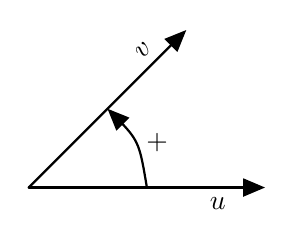
\begin{tikzpicture}[line cap=round,line join=round,>=triangle 45,scale=1,font=\normalsize]
    \draw[thick,->] (0,0) -- (3,0) node[pos=0.8, below] {$u$};
    \draw[thick,->] (0,0) -- (2,2) node[pos=0.8, sloped, above] {$v$};
    \draw[thick,->] (1.5,0) .. controls(1.4, 0.6) ..  (1, 1) node[pos=0.5, right] {$+$};
  \end{tikzpicture}
\end{center}
\begin{prz}
  Para $(u,v)$ jest dodatnio zorientowana.
\end{prz}

Wartość bezwzględna wyznacznika równa jest polu równoległoboku rozpinanego przez parę wektorów, skąd możemy otrzymać drugą (równoważną) definicję wyznacznika:
\begin{df}(geometryczna) $\forall u,v\in\RR^2$: $$\det(u,v) = \norm{u}\norm{v}\sin\sphericalangle(u,v).$$ \end{df}

\begin{ft}
    Pole dowolnego wielokąta w $\RR^2$ (w którym kolejnie wierzchołki to $v_0,v_1, \dots v_{n-1})$ można wyliczyć za pomocą wzoru: 
        $$ \sum_{k=1}^{n-1} \det(v_{k \ mod \ n},v_{k+1 \ mod \ n})$$
\end{ft}

\end{document}
